\documentclass[pdf]{beamer}
\usepackage[utf8]{inputenc}
\usepackage{amsmath}
\usepackage{amsfonts}
\usepackage{amssymb}
\usepackage{graphicx}
\usepackage{animate}
\usepackage{multimedia}
\usepackage[ruled, vlined, boxed]{algorithm2e}
\usetheme{metropolis}
\mode<presentation>{}

\title{Analysis of Boundary Trees and Differentiable Boundary Trees}
%\subtitle{}
\author{Jay Ricco, David Van Chu}
\institute{Wentworth Institute of Technology}
\date{August 8, 2017}
\begin{document}
	
	% Title 
	\begin{frame}
		\titlepage
	\end{frame}

	% Introduction
	\begin{frame}
		\frametitle{Introduction}
		The goal of this project was to understand, evaluate, and further study the properties of the Boundary Tree\footnote[1]{https://www.aaai.org/ocs/index.php/AAAI/AAAI15/paper/viewFile/9848/9953} and Differentiable Boundary Tree\footnote[2]{https://arxiv.org/abs/1702.08833} algorithms, presented in their respective papers, \textit{The Boundary Forest Algorithm for Online Supervised and Unsupervised Learning}, and \textit{Learning Deep Nearest Neighbor Representations Using Differentiable Boundary Trees}.\\ 
		
	\end{frame}

	% Boundary Trees
	\section{Boundary Trees}
	\begin{frame}
		\frametitle{BT's - Introduction}
		
		\begin{itemize}
			\item Learning Domain - Classification (Supervised)
			\item Goal - Fast to train, fast to query , on-line, instance based learning algorithm that can adapt to complex data distributions.
			\item Allows for data to self-distribute given distance and class.
		\end{itemize}
	\end{frame}

	\begin{frame}
		\frametitle{BT's - Querying Procedure}
		\begin{algorithm}[H]
			\Begin(BTQuery\text{($\mathbf{x}$)}){%
				\KwIn{$\mathbf{x}$ - the query feature vector.}
				\KwOut{$\mathtt{closest}$- closest node in the boundary tree.}
				Initialize $\mathtt{current}$ to root node. \\
				\While{True}{
					Let $N$ be the set of child nodes of $\mathtt{current}$.\\
					\If{$|N| < k$}{$N\, +=\, $\{$v$\}}
					$\mathtt{closest} = \arg\min_{\mathbf{x_c}\, \in\, N} d(\mathbf{x_c}, \mathbf{x})$\\
					\If{$\mathtt{closest} = \mathtt{current}$}{\textbf{break}\\}
					$\mathtt{current} \leftarrow \mathtt{closest}$\\
				}
			}
		\end{algorithm}
	\end{frame}
	\begin{frame}
	\frametitle{BT's - Training Procedure}
	\begin{algorithm}[H]
		
		\Begin(BTTrain\text{($\mathbf{x},\ \mathbf{y}$)}){%
			\KwIn{$\mathbf{x}$ - the new examples feature vector.}
			\KwIn{$\mathbf{y}$ - the new examples target class.}
			Initialize $\mathtt{closest} = \mathsf{BTQuery(\mathbf{x})}$\\
			\If{$\mathtt{closest}.y \ne \mathbf{y}$}
			{
				Create node $\mathtt{v}_{new}$ in the Boundary Tree with position $\mathbf{x}$ and target class $\mathbf{y}$.\\
				Add a new edge from $\mathtt{closest} \rightarrow \mathtt{v}_{new}$.\\
			}
		}
	\end{algorithm}
	\end{frame}

	\begin{frame}
		\frametitle{BT's - Testing and Data}
		Our implementation of the algorithm was tested using three data sets:
		\begin{itemize}
			\item MNIST\\
			\item CIFAR-10\\
			\item Ground-Truth\\
		\end{itemize}
		Initial observations indicated that:\\
		\begin{enumerate}
		 	\item the max. branching factor value ($k$) is crucial with respect to the performance of the algorithm on a given data set.\\
		 	\item While the total testing time and accuracy plateau, with $\uparrow$ examples, training time $\in\ \mathcal{O}\left(n\right)$.
		 	\item BT's perform far better with MNIST than CIFAR; this shows inadequacy of the Euclidean distance metric for high feature complexity use-cases.
		 \end{enumerate}
	\end{frame}
\begin{frame}
\frametitle{BT's - Testing and Data (MNIST Example)}
	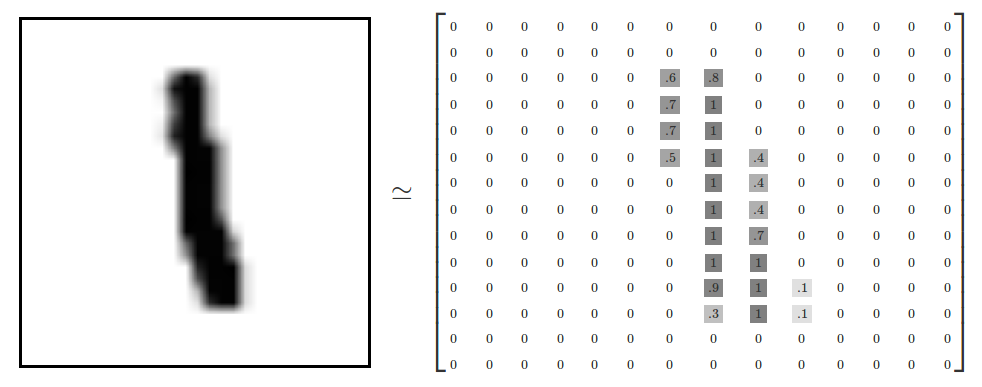
\includegraphics[scale=0.3]{./Graphics/MNIST-Matrix}
\end{frame}
\begin{frame}
\frametitle{BT's - Testing and Data (CIFAR Example)}
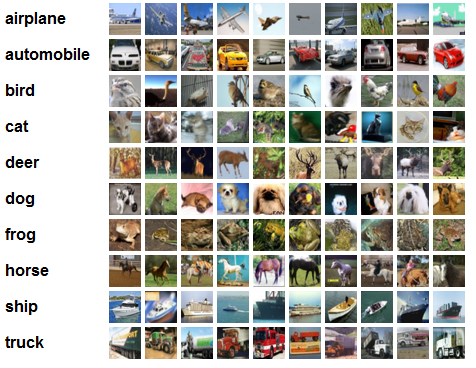
\includegraphics[scale=0.7]{./Graphics/cifar_preview}
\end{frame}
	\begin{frame}
	\frametitle{BT Observations - MNIST}
		\begin{table}
			\begin{tabular}{|c|c|c|c|}
				\hline 
				\rule[-1ex]{0pt}{2.5ex} \textbf{k} & \textbf{Training Time (s)} & \textbf{Testing Time (s)} & \textbf{Accuracy (\%)} \\ 
				\hline 
				\rule[-1ex]{0pt}{2.5ex} 2 & 75.96443768
 & 14.89228232 & 79.248 \\ 
				\hline 
				\rule[-1ex]{0pt}{2.5ex} 3 & 76.26015964 & 14.11042054 & 82.253 \\ 
				\hline 
				\rule[-1ex]{0pt}{2.5ex} 5 & 72.54322867 & 14.19308667 & 84.988 \\ 
				\hline 
				\rule[-1ex]{0pt}{2.5ex} 10 & 93.82171679 & 18.15971713 & 87.397 \\ 
				\hline 
				\rule[-1ex]{0pt}{2.5ex} 20 & 128.2968537 & 25.59608793 & 88.211 \\ 
				\hline 
				\rule[-1ex]{0pt}{2.5ex} 50 & 165.1073234 & 34.94613609 & 88.036 \\ 
				\hline 
				\rule[-1ex]{0pt}{2.5ex} 100 & 164.9357249 & 35.71075509 & 87.952 \\ 
				\hline 
				\rule[-1ex]{0pt}{2.5ex} $\infty$ & 167.4871073 & 36.10234139 & 87.952 \\ 
				\hline 
			\end{tabular} 
			\caption{For each test the branching factor is changed, and each data point was acquired by taking an average over 10 runs.}
		\end{table}
	\end{frame}

	\begin{frame}
	\frametitle{BT Observations - CIFAR-10}
		\begin{table}
			\begin{tabular}{|c|c|c|c|}
				\hline 
				\rule[-1ex]{0pt}{2.5ex} \textbf{k} & \textbf{Training Time (s)} & \textbf{Testing Time (s)} & \textbf{Accuracy (\%)} \\ 
				\hline 
				\rule[-1ex]{0pt}{2.5ex} 2 & 31.6216013
 & 10.17820182 & 23.928 \\ 
				\hline 
				\rule[-1ex]{0pt}{2.5ex} 3 & 28.85782518 & 9.416226149 & 25.422 \\ 
				\hline 
				\rule[-1ex]{0pt}{2.5ex} 5 & 32.36283786 & 10.46060543 & 26.509 \\ 
				\hline 
				\rule[-1ex]{0pt}{2.5ex} 10 & 36.72829039 & 12.98402145 & 27.169 \\ 
				\hline 
				\rule[-1ex]{0pt}{2.5ex} 20 & 51.99976389 & 18.622286033 & 27.708 \\ 
				\hline 
				\rule[-1ex]{0pt}{2.5ex} 50 & 79.45825586 & 29.97079742 & 27.453 \\ 
				\hline 
				\rule[-1ex]{0pt}{2.5ex} 100 & 98.72666419& 38.09738462 & 27.629 \\ 
				\hline 
				\rule[-1ex]{0pt}{2.5ex} $\infty$ & 125.9124599 & 54.22032864 & 27.283 \\ 
				\hline 
			\end{tabular} 
			\caption{For each test the branching factor is changed, and each data point was acquired by taking an average over 10 runs. Notice how low the accuracy is. }
		\end{table}
	\end{frame}
	\begin{frame}
		\frametitle{BT Observations - CIFAR-10 (cont.)}
		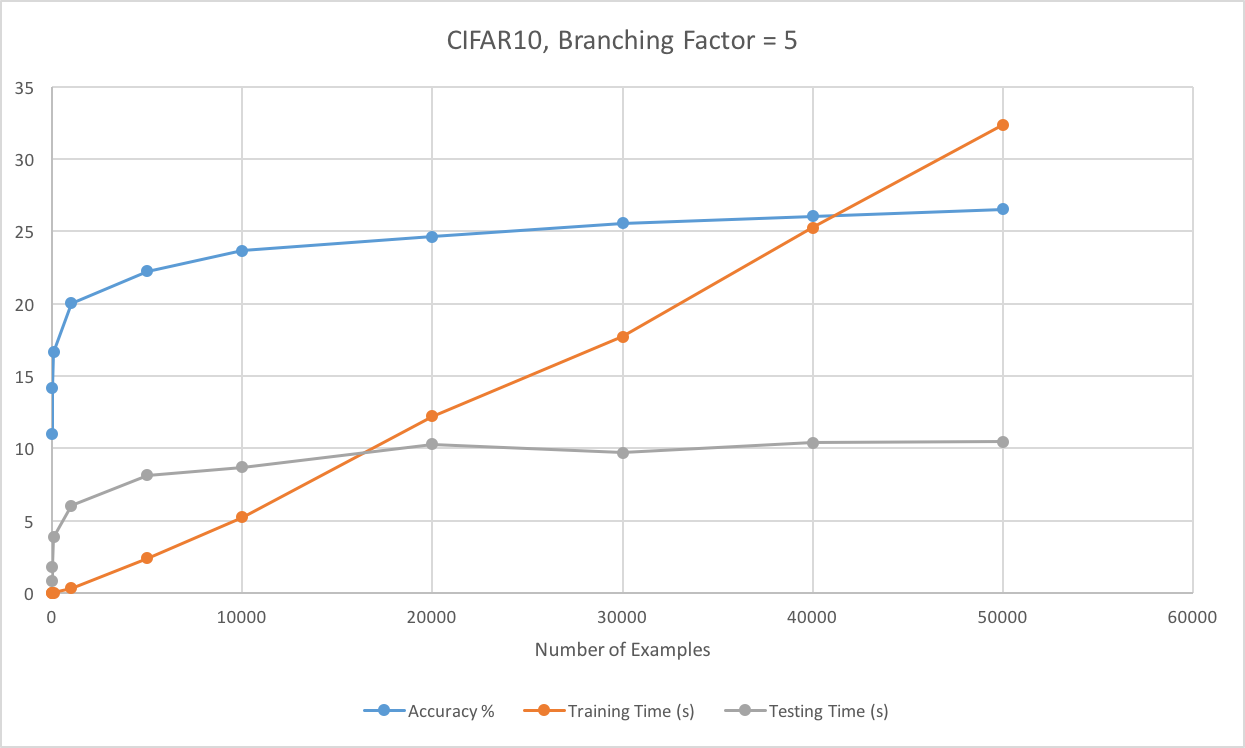
\includegraphics[scale=0.5]{Graphics/CIFAR_k5}
	\end{frame}
	\begin{frame}
		\frametitle{BT Observations - CIFAR-10 (cont.)}
		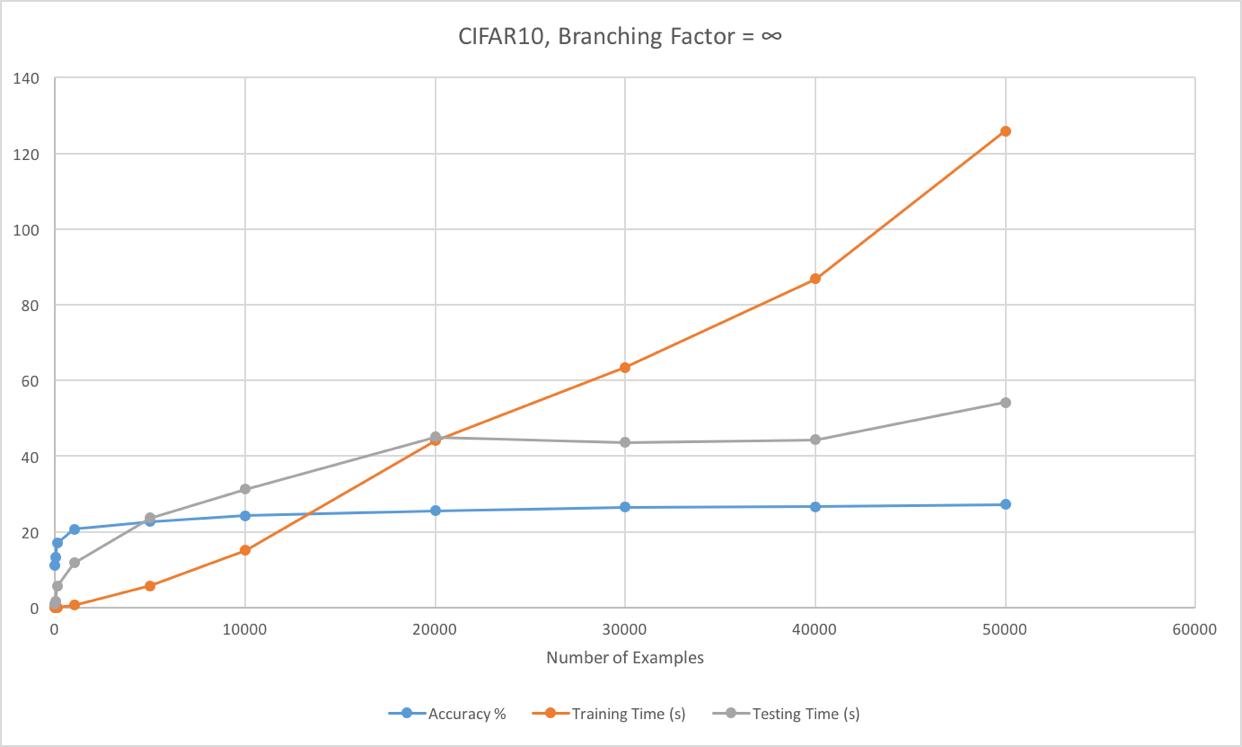
\includegraphics[scale=0.5]{Graphics/CIFAR_kinf}
	\end{frame}

	% Differentiable Boundary Trees
	\section*{Differentiable Boundary Trees}
	\begin{frame}
		\frametitle{DBT's - Introduction}
		
		\textbf{Key Difference}: DBT's are augmented with a neural network that learns the \textit{best} transform to apply on input features to maximize the L$^2$ distance between any two examples of different classes in the output space.\\
		
		The algorithm dynamically builds neural networks which calculate the probabilities of an example being a specific class. This dynamically build network is then back-propagated through all the operations performed on it, distributing error to the proper parameters. 

	\end{frame}
	\begin{frame}
	\frametitle{DBT's - Probabilistic Modeling of Traversals}
		\begin{itemize}
			\item {In order for any gradient-based machine learning method to work, there must be a hypothesis function, and it must be completely differentiable.}
			\item {Trees are inherently discrete, and we're traversing them layer-by-layer...}
			\item {How do we make our hypothesis differentiable?}
		\end{itemize}
	\end{frame}
	\begin{frame}
		\frametitle{DBT's - Probabilistic Modeling of Traversals}
		\begin{itemize}
			\item Let's start by giving a firm definition to the distance function:
				$$d(x_1, x_2) = \sqrt{\sum_{k}\left(x_{1, k} - x_{2, k}\right)^2}$$\\
			\item With that defined, the probability of transitioning from a parent node to itself or any of it's children is: 
			$$ p(\mathbf{x_i} \rightarrow \mathbf{x_j} | \mathbf{x_{query}}) = \mathsf{SoftMax}_{i, j \in child(i)}\left(-d(\mathbf{x_j}, \mathbf{x_{query}})\right)$$
			$$ = \dfrac{\exp(-d(\mathbf{x_j}, \mathbf{x_{query}}))}{
			\sum_{j' \in (i, j \in child(i))} \exp(-d(\mathbf{x_{j'}}, \mathbf{x_{query}}))}$$
			\item Computing the full $P(path | \mathbf{x_{query}})$ distribution is hard; so we approximate the path through the tree, for some $\mathbf{x_{query}}$ by greedily selecting nodes at each level with the maximum calculated probability; this gives us the approximate path, $path*$.
		\end{itemize}
	\end{frame}
		\begin{frame}
	\frametitle{DBT's - Final Class Probabilities}
	\begin{itemize}
		\item The full equation to calculate the log class probabilities is as follows:
		$$ \log p(c |f_{\theta}(\mathbf{x_{query}})) = \sum_{\mathbf{x_i} \rightarrow \mathbf{x_j} \in path^{*} | \mathbf{x_{query}}} \log p(f_{\theta}(\mathbf{x_i}) \rightarrow f_{\theta}(\mathbf{x_j}) | f_{\theta}(\mathbf{x_{query}}))$$
		$$ + \log \sum_{\mathbf{x_k} \in \mathsf{sibling}(\mathbf{x_{final}})} p(\mathsf{parent}(f_{\theta}(\mathbf{x_k})) \rightarrow f_{\theta}(\mathbf{x_k}) | f_{\theta}(\mathbf{x_{query}}))c(\mathbf{x_k})$$
		\item In other words, apply the transform to all the relevant feature vectors, then use the greedy path technique to calculate the log-class probabilities up until the last transition. At this point, all of the transitions to possible leaves are averaged over. 
	\end{itemize}
	\end{frame}

\begin{frame}
\frametitle{DBT's - Final Class Probabilities}
	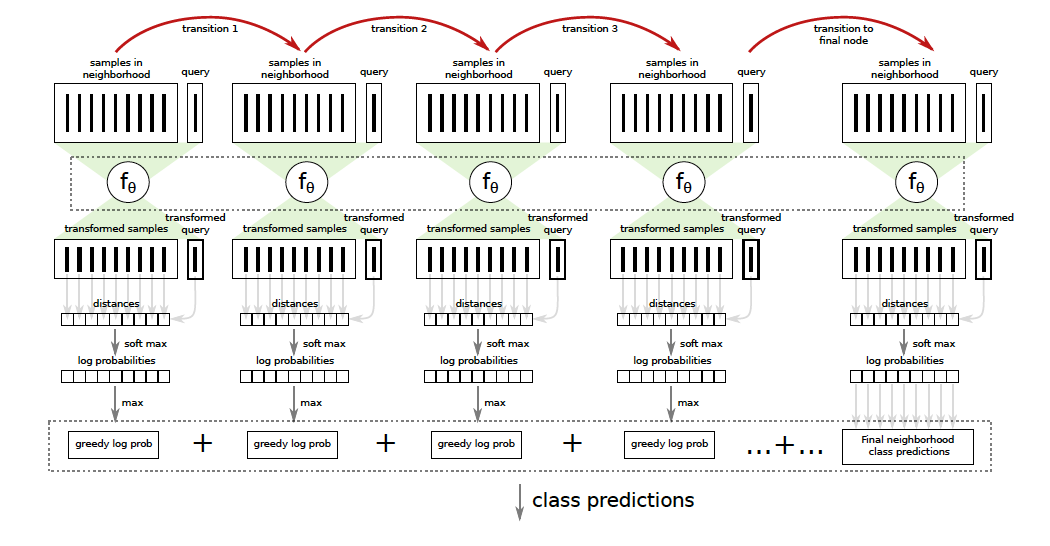
\includegraphics[scale=0.59]{Graphics/papershot}
\end{frame}

\begin{frame}
\frametitle{DBT's -  Problems}
\begin{itemize}
	\item Dynamic network = Dynamic computation.
	\item The time it takes to perform a training batch is relatively constant, but the time to convergence is \textit{large}. (For reference, one MNIST test took 30 hours!)
	\item Removes the whole point of having an on-line, fast, incremental learning algorithm. 
\end{itemize}
\end{frame}
\begin{frame}
\frametitle{DBT's -  MNIST Data Set}
	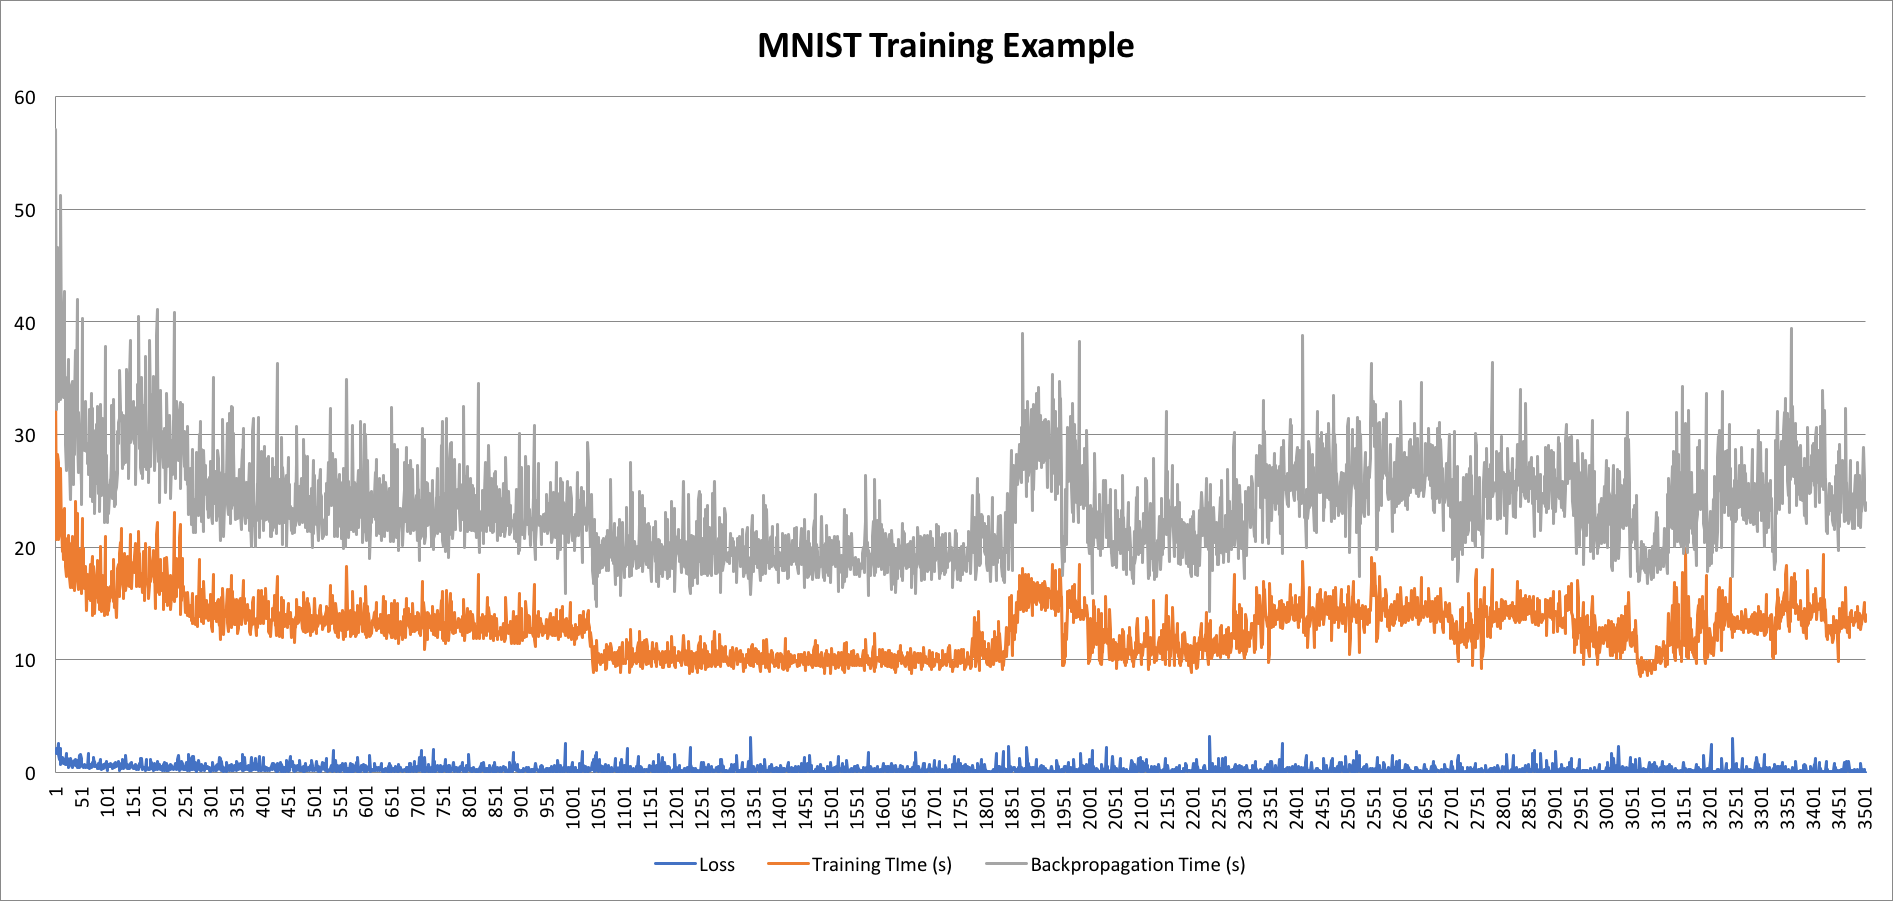
\includegraphics[scale=0.36]{./Graphics/mnist1}
\end{frame}

\begin{frame}
\frametitle{DBT's -  Half Moon Data Set}
	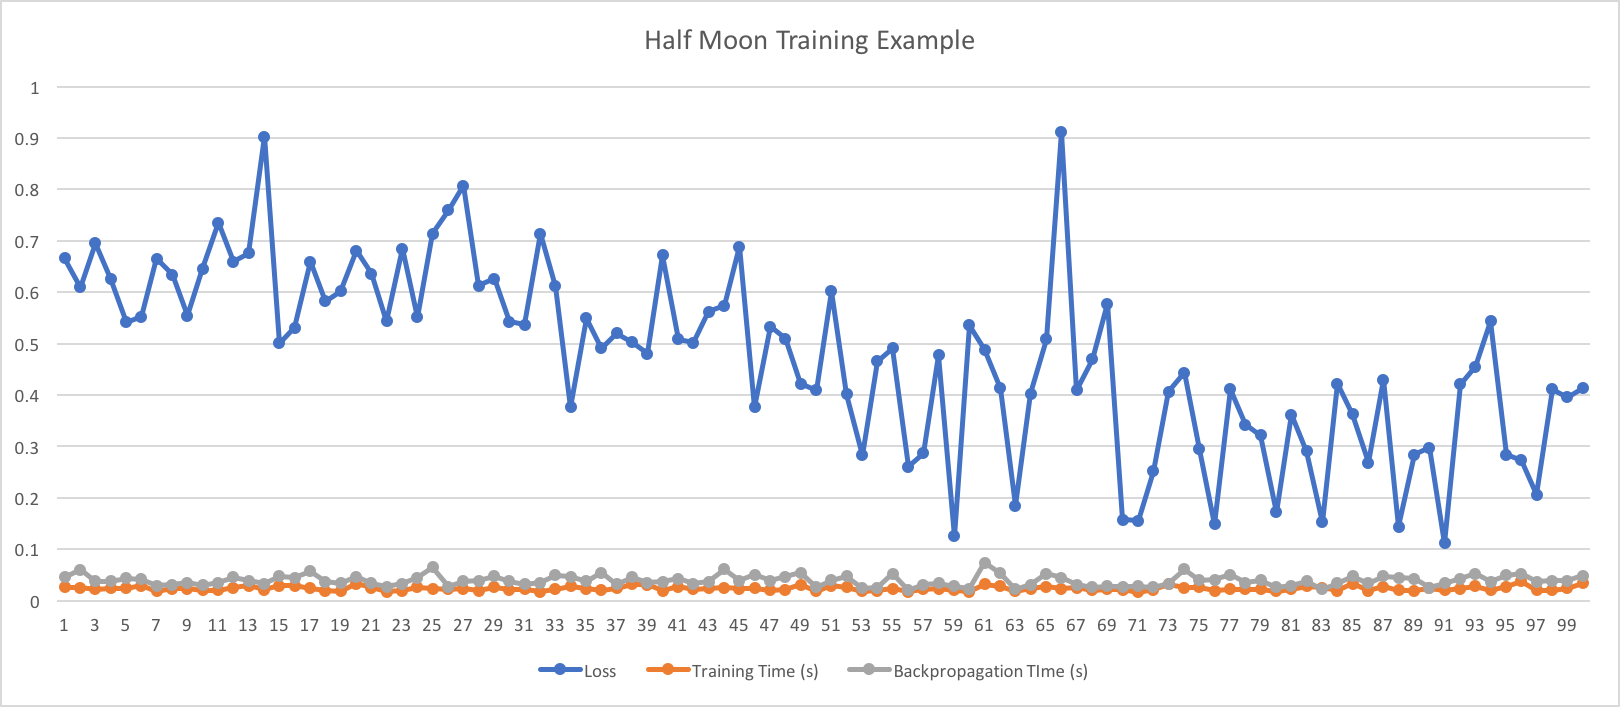
\includegraphics[scale=0.4]{./Graphics/HalfMoon1}
\end{frame}

\begin{frame}
	\frametitle{DBT's - Conclusions}
	\begin{itemize}
		\item Ideal next steps would be to figure out a way to parallelize training. 
		\item Otherwise, this method has limited usability due to time. (A standard neural network would do well enough.)
		\item Bogosort would be faster. 
	\end{itemize}
\end{frame}

\end{document}